\documentclass[11pt,a4paper]{article}

% ─── Packages ───
\usepackage[margin=2.2cm]{geometry}
\usepackage{graphicx}
\usepackage{booktabs}
\usepackage{hyperref}
\usepackage{xcolor}
\usepackage{enumitem}
\usepackage{tabularx}
\usepackage{float}
\usepackage{caption}
\usepackage{amsmath}

% Overfull hbox prevention
\tolerance=1000
\emergencystretch=3em
\hfuzz=2pt

% Hyperlink styling
\hypersetup{colorlinks=true, linkcolor=blue!60!black, citecolor=blue!60!black, urlcolor=blue!60!black}

% Code-like formatting for inline tokens
\newcommand{\tok}[1]{\texttt{#1}}

\title{\textbf{Meta-CoT Control-V5:\\From Metacognitive Detection to Execution}}
\author{Seungpil Lee}
\date{April 4, 2026}

\begin{document}
\maketitle

\begin{abstract}
The Control-V5 experiment series trains Qwen3-8B to emit structured metacognitive control signals (\tok{<|meta|>} blocks) and evaluates whether these signals translate into measurable OOD test-time adaptation gains. Eleven model variants were evaluated on a pilot set of 90 problems. Meta-CoT signals are parseable and trainable via reward shaping, but the current rewards do not produce functional test-time controllers. The bottleneck has shifted from meta detection to meta execution: models diagnose weaknesses but fail to act on them. Three targeted fixes are proposed for the next round.
\end{abstract}

\tableofcontents
\newpage

% ──────────────────────────────────────────────────────────────────────
\section{Executive Summary}

\begin{table}[H]
\centering
\caption{Key model comparison (n=90 pilot, 30 per benchmark)}
\label{tab:exec-summary}
\begin{tabular}{lccccl}
\toprule
Model & Acc & ECE & Conf\_Cov & Wrong\_Hi & Key Observation \\
\midrule
base\_sft & 42.2 & n/a & 0.0 & n/a & Accuracy baseline; no meta \\
E9 & 41.1 & 0.301 & 91.1 & 50.9 & Highest meta acc; verify decorative \\
E8 & 38.9 & 0.322 & 23.3 & 3.6 & Overconf suppression works \\
E5 & 40.0 & 0.790 & 1.1 & 0.0 & Reward escape via omission \\
\bottomrule
\end{tabular}
\end{table}

\textbf{Conclusion.} Meta-CoT signals are parseable and trainable via reward shaping, but the current generation of rewards does not produce functional test-time controllers. The primary bottleneck has shifted from \emph{meta detection} to \emph{meta execution}: models diagnose weaknesses but fail to act on them. Three targeted fixes---same-route repetition penalty, route-switch evidence reward, and confidence omission floor---are proposed for the next round.

% ──────────────────────────────────────────────────────────────────────
\section{Background and Intent}

\subsection{Definition: Meta-CoT}

Meta-CoT is a structured reasoning protocol in which a language model interleaves standard chain-of-thought computation with explicit metacognitive control blocks delimited by \tok{<|meta|>} and \tok{<|/meta|>} tokens. Each meta block contains three fields:

\begin{itemize}[nosep]
  \item \textbf{confidence}: a scalar in $[0, 1]$ representing the model's posterior belief in the current solution route.
  \item \textbf{assessment}: a natural-language diagnosis of why the current route may be incorrect.
  \item \textbf{action}: one of \{verify, redirect, diagnose\}, specifying the next controller step.
\end{itemize}

The term \textbf{controller} refers to the decision function that maps the current reasoning state to one of these actions. A functional controller would (a)~detect when confidence is unjustified, (b)~invoke verify with an independent check rather than a paraphrase, and (c)~execute redirect by switching the solution route when diagnosis indicates a dead end.

\subsection{Research Questions}

\begin{itemize}[nosep]
  \item \textbf{RQ1 (Parseability and Adaptation):} Can Meta-CoT teach a parseable controller state that enables OOD test-time adaptation?
  \item \textbf{RQ2 (Learnability via Rewards):} Can Meta-RL make verify, redirect, and diagnosis behaviors learnable through reward decomposition?
  \item \textbf{RQ3 (Curriculum Extensibility):} Can curriculum/RAG extend from reliable diagnosis to improved performance?
\end{itemize}

\subsection{Experimental Context}

All models are fine-tuned from a Qwen3-8B base. SFT variants use supervised fine-tuning on 4,996 Meta-CoT chains generated by GPT-5.4-mini. RL variants apply GRPO with decomposed reward functions. Evaluation uses \tok{max\_tokens=4096}.

% ──────────────────────────────────────────────────────────────────────
\section{Experiment Design}

\subsection{Reward Decomposition Contract}

The RL experiments form a progression from broad to targeted rewards:

\paragraph{E3: Full Meta + Correctness + Calibration.}
\textbf{Intent:} Combine all reward components.
\textbf{Hypothesis:} Joint optimization will produce an emergent controller.
\textbf{Verification:} Accuracy $\geq$ base\_sft; ECE $<$ 0.3; Wrong\_Hi $<$ 20\%.

\paragraph{E5: Correctness-Only RL.}
\textbf{Intent:} Remove all meta rewards.
\textbf{Hypothesis:} Without meta rewards, no meta blocks emitted; accuracy preserved.
\textbf{Verification:} Accuracy $\geq$ base\_sft; Conf\_Cov $\approx$ 0.

\paragraph{E8: Overconfidence Penalty + Correctness.}
\textbf{Intent:} Penalize high-confidence wrong answers.
\textbf{Hypothesis:} Wrong\_Hi will decrease without destroying accuracy.
\textbf{Verification:} Wrong\_Hi $<$ 10\%; accuracy within 3\%p of base\_sft.

\paragraph{E9: Verify Reward + Correctness.}
\textbf{Intent:} Reward verify actions on uncertain completions.
\textbf{Hypothesis:} Verify frequency and accuracy will improve.
\textbf{Verification:} Conf\_Cov $>$ 80\%; AIME improvement.

\paragraph{E10: Full Controller (Verify + Redirect + Diagnosis).}
\textbf{Intent:} Train the complete metacognitive controller.
\textbf{Hypothesis:} Full reward stack produces detect--diagnose--recover behavior.
\textbf{Verification:} Accuracy $\geq$ base\_sft; diagnosis-to-recovery $>$ 50\%.

\subsection{SFT Ablations}

\begin{table}[H]
\centering
\begin{tabular}{ll}
\toprule
Model & Training Data \\
\midrule
all\_sft & Full Meta-CoT with verify + redirect + diagnosis \\
verify\_sft & Chains containing only verify meta blocks \\
redirect\_sft & Chains containing only redirect meta blocks \\
\bottomrule
\end{tabular}
\end{table}

% ──────────────────────────────────────────────────────────────────────
\section{Quantitative Results}

\subsection{Control-V5 Pilot (n=90)}

\begin{table}[H]
\centering
\caption{Full pilot results (30 problems per benchmark)}
\label{tab:pilot-full}
\small
\begin{tabular}{lccccccc}
\toprule
Model & Acc & AIME & GSM8K & MATH500 & Conf\_Cov & ECE & Wrong\_Hi \\
\midrule
base\_sft     & 42.2 & 13.3 & 80.0 & 33.3 & 0.0   & n/a   & n/a \\
all\_sft      & 33.3 & 6.7  & 63.3 & 30.0 & 88.9  & 0.398 & 51.7 \\
verify\_sft   & 36.7 & 3.3  & 66.7 & 40.0 & 82.2  & 0.492 & 80.7 \\
redirect\_sft & 35.6 & 10.0 & 63.3 & 33.3 & 48.9  & 0.160 & 0.0 \\
E3            & 30.0 & 3.3  & 63.3 & 23.3 & 100.0 & 0.515 & 71.4 \\
E5            & 40.0 & 3.3  & 80.0 & 36.7 & 1.1   & 0.790 & 0.0 \\
E8            & 38.9 & 10.0 & 80.0 & 26.7 & 23.3  & 0.322 & 3.6 \\
E9            & 41.1 & 6.7  & 90.0 & 26.7 & 91.1  & 0.301 & 50.9 \\
E9b           & 40.0 & 6.7  & 83.3 & 30.0 & 0.0   & n/a   & n/a \\
E9c           & 36.7 & 6.7  & 73.3 & 30.0 & 7.8   & 0.264 & 1.8 \\
E10           & 35.6 & 6.7  & 66.7 & 33.3 & 5.6   & 0.340 & 0.0 \\
\bottomrule
\end{tabular}
\end{table}

\begin{figure}[H]
\centering
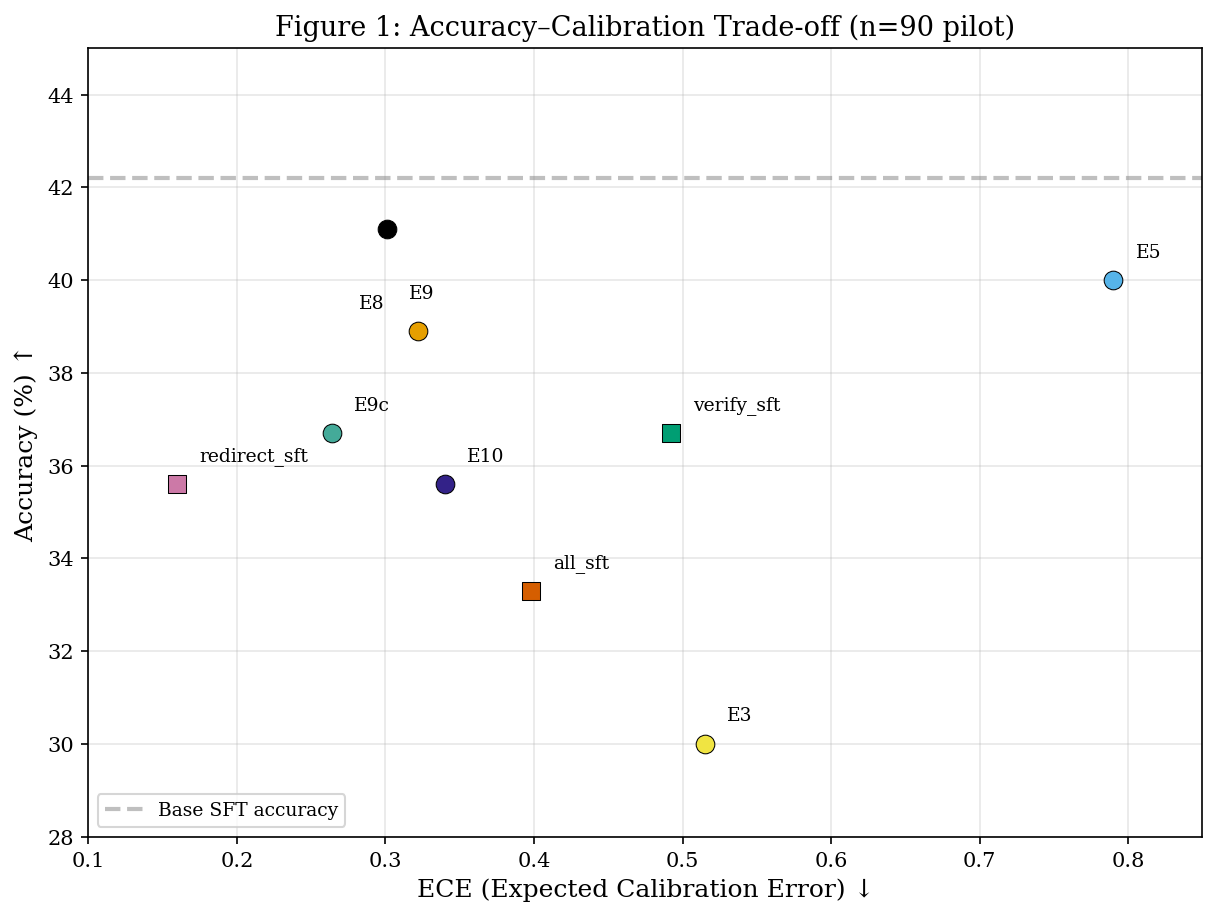
\includegraphics[width=0.85\textwidth]{figures/fig1_accuracy_vs_ece.png}
\caption{Accuracy--Calibration trade-off. Models with ECE defined (Conf\_Cov $>$ 0) plotted. Dashed line = base\_sft accuracy.}
\label{fig:acc-ece}
\end{figure}

\textbf{Key observations:}
\begin{enumerate}[nosep]
  \item No meta model exceeds base\_sft accuracy (42.2). The highest meta model is E9 at 41.1.
  \item E8 achieves Wrong\_Hi $<$ 10\% (3.6\%) while maintaining accuracy within 3.3\%p of base\_sft.
  \item E3 shows the worst accuracy (30.0) despite 100\% confidence coverage.
  \item E5, E9b, and E10 have confidence coverage below 10\%, rendering calibration metrics unreliable.
\end{enumerate}

\subsection{Per-Benchmark Analysis}

E9 achieves 90.0 on GSM8K (highest in pilot), indicating verify rewards can improve arithmetic self-checking. However, E9 scores only 26.7 on MATH-500, suggesting verify does not transfer to harder reasoning. AIME is the hardest benchmark, and meta overhead actively harms performance: only base\_sft achieves 13.3.

\begin{figure}[H]
\centering
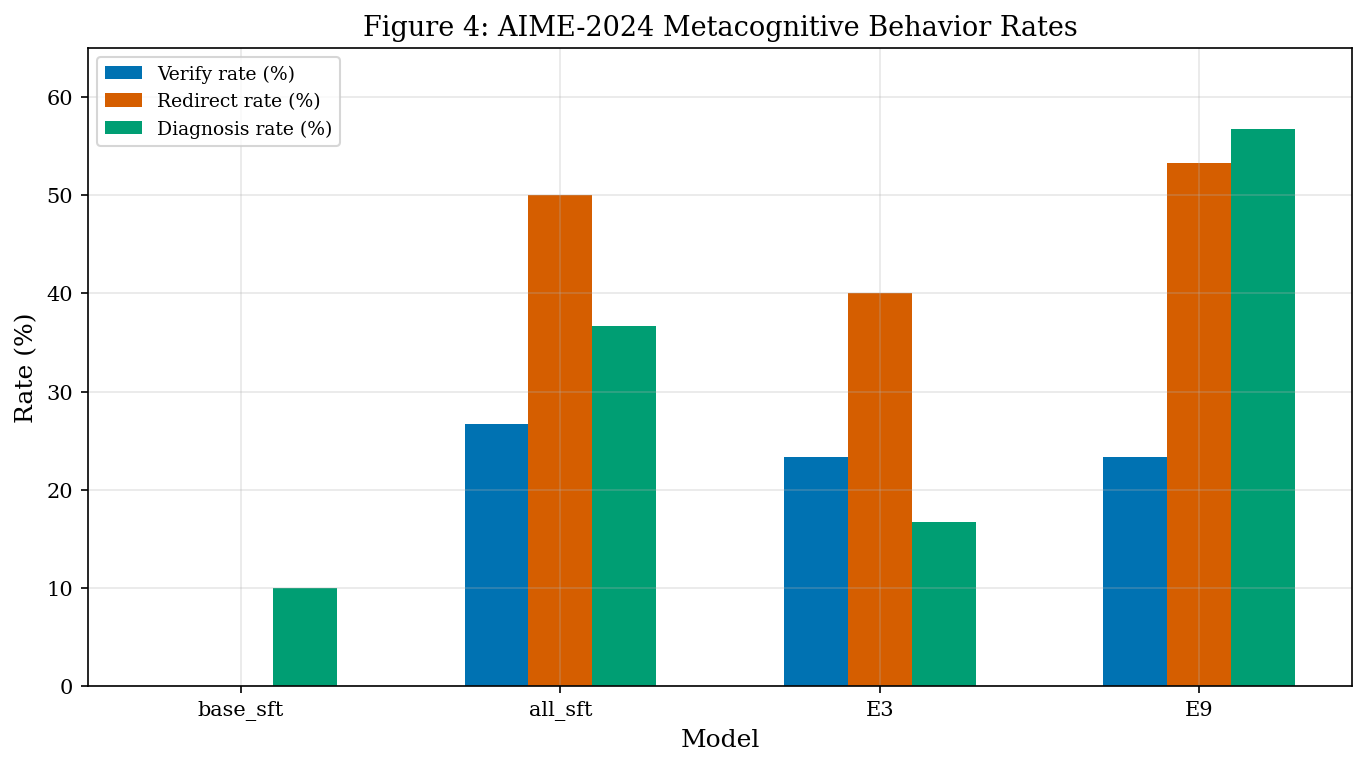
\includegraphics[width=0.85\textwidth]{figures/fig4_aime_behavior.png}
\caption{AIME-2024 metacognitive behavior rates across selected models.}
\label{fig:aime-behavior}
\end{figure}

\subsection{Large-Scale Reference (1,030 problems)}

\begin{table}[H]
\centering
\caption{Previous-round 1,030-problem evaluation}
\begin{tabular}{lc}
\toprule
Model & Overall Accuracy \\
\midrule
V2 SFT & 72.72\% \\
V3 SFT & 72.0\% \\
E5 & 72.04\% \\
Base SFT & 71.7\% \\
E8 & 67.2\% \\
\bottomrule
\end{tabular}
\end{table}

\begin{figure}[H]
\centering
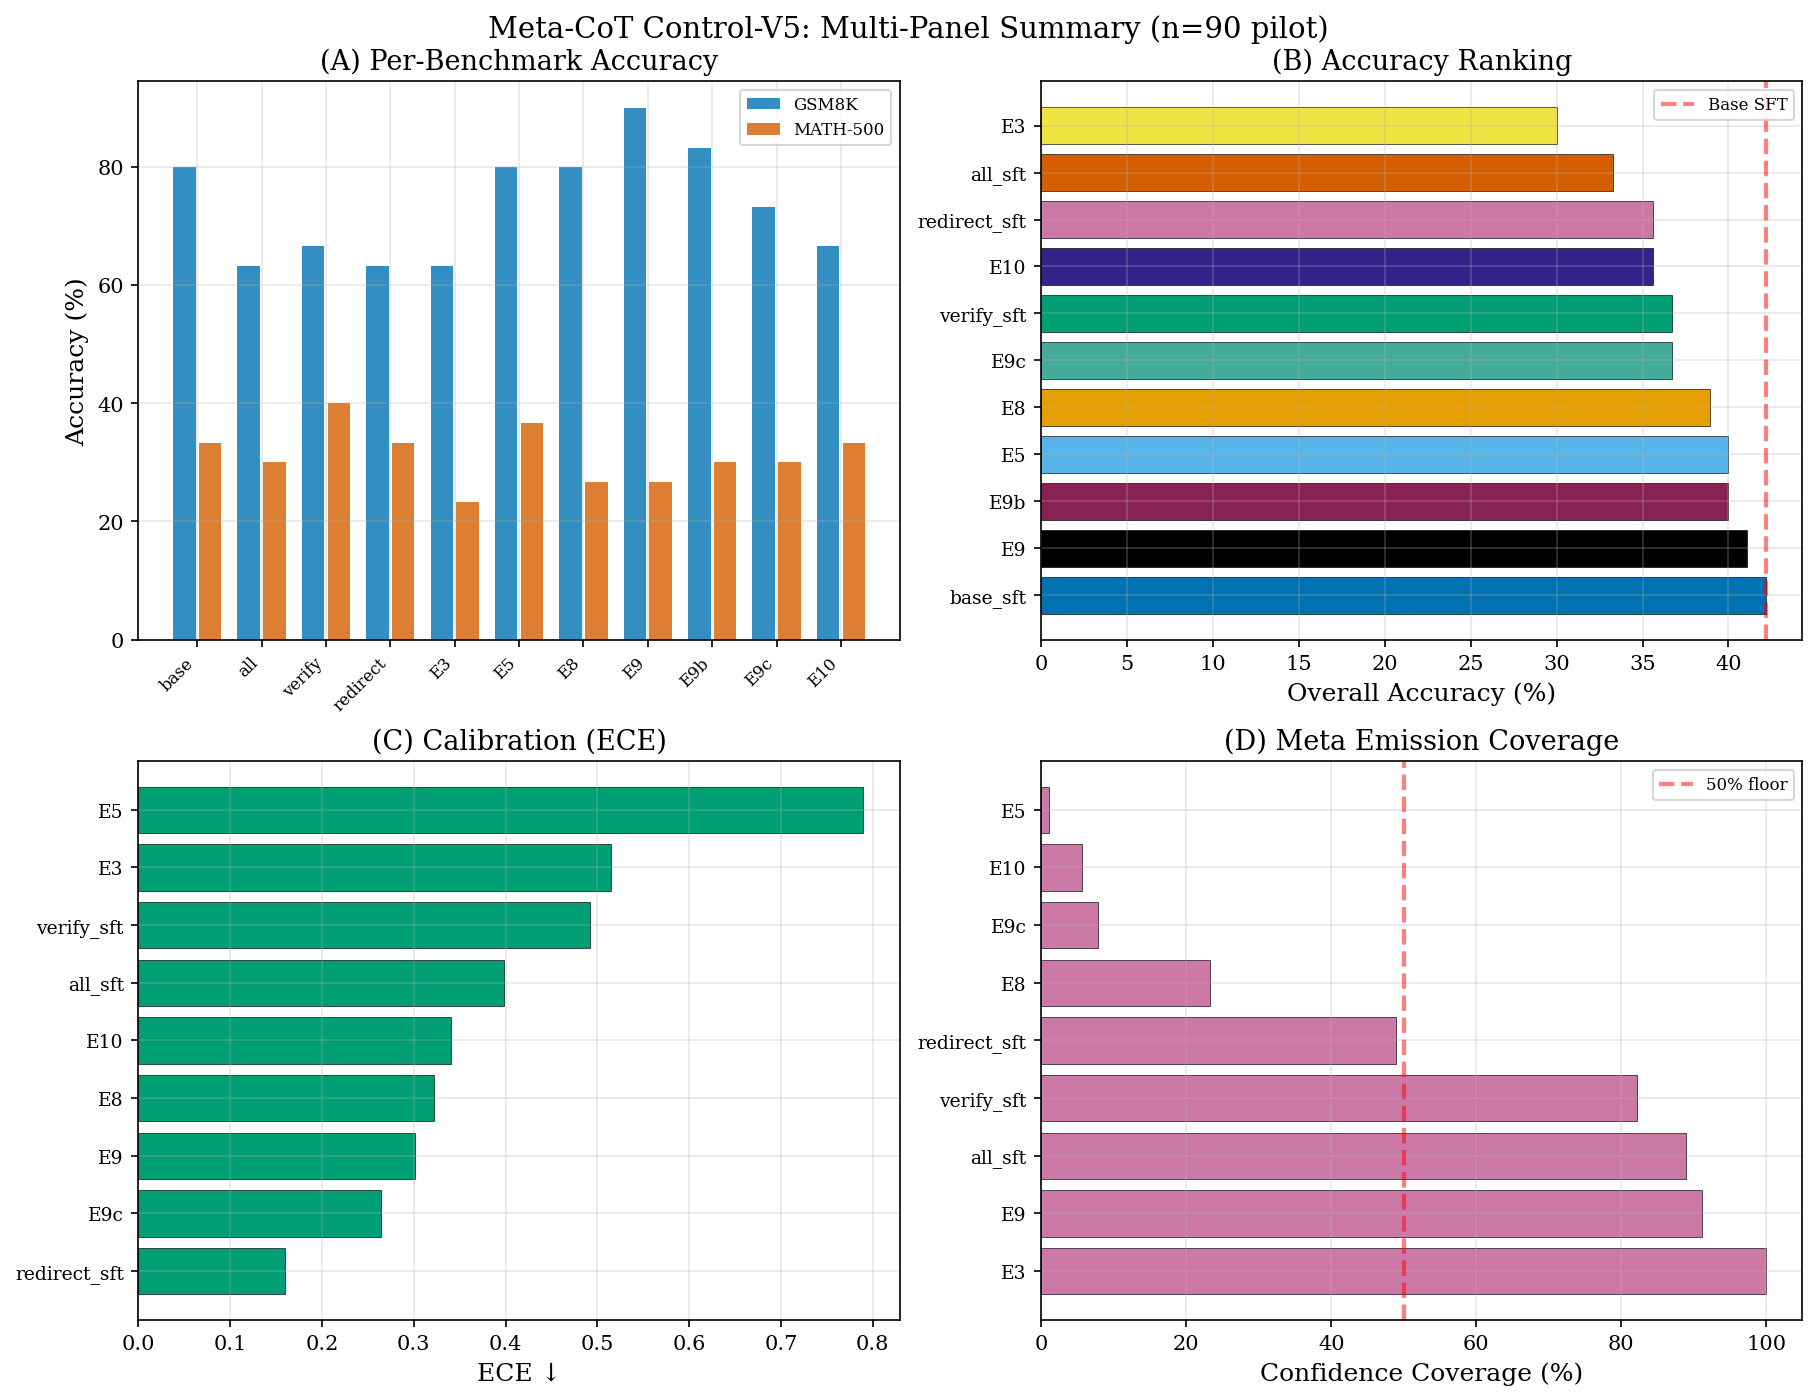
\includegraphics[width=\textwidth]{figures/fig5_multipanel_summary.png}
\caption{Multi-panel summary: (A) per-benchmark accuracy, (B) overall ranking, (C) ECE, (D) confidence coverage.}
\label{fig:multipanel}
\end{figure}

% ──────────────────────────────────────────────────────────────────────
\section{Qualitative Failure Analysis}

Failure modes were identified by manual inspection of wrong-answer completions (source: \tok{failure\_analysis\_2026\_04\_04.json}).

\subsection{Overconfident Verify Failed}

\textbf{Affected models:} E3 (45 cases), E9 (15 cases), verify\_sft.

The model completes an initial solution, emits a meta block stating ``single route, should verify,'' then re-derives the same calculation using identical assumptions. Confidence remains high (0.86--0.89). The verification step produces a \emph{paraphrase} of the original reasoning rather than an independent falsification.

\textbf{Example (E3, GSM8K, ``sheep counting''):} The model computes total $= 160 + 80 + 20 = 320$. Meta block: ``confidence: 0.88. I should do a brief independent check.'' Verification: recalculates $20 + 80 + 160 = 320$. Answer remains 320 (wrong; correct = 260).

\textbf{Root cause:} The verify reward triggers on verification \emph{language}, not verification \emph{independence}.

\subsection{Diagnosis Without Recovery}

\textbf{Affected models:} E8 (4 cases), E10 (1 case), E3 (4 cases).

The meta block correctly identifies the weakness and specifies a \tok{study\_need}. However, the subsequent reasoning continues along the original route without executing the switch.

\textbf{Example (E10, AIME ``Aimeville sets''):} Meta diagnoses need for inclusion-exclusion. Subsequent reasoning: ``437 + 234 + x = 900, x = 229.'' No inclusion-exclusion attempted. (Correct answer: 73.)

\textbf{Root cause:} The redirect reward credits diagnosis text without requiring execution evidence.

\subsection{Single Intervention Only}

\textbf{Affected:} all\_sft, E8, E10. A single meta block appears early; no further monitoring follows, even on hard problems.

\textbf{Root cause:} Reward functions do not incentivize repeated intervention.

\subsection{Reward Escape via Confidence Omission}

\textbf{Affected:} E5 (54 cases), E10 (53 cases). The model omits meta blocks entirely, avoiding calibration penalties.

\textbf{Root cause:} The calibration reward returns 0.0 (neutral) for missing confidence, making omission cost-free.

\begin{figure}[H]
\centering
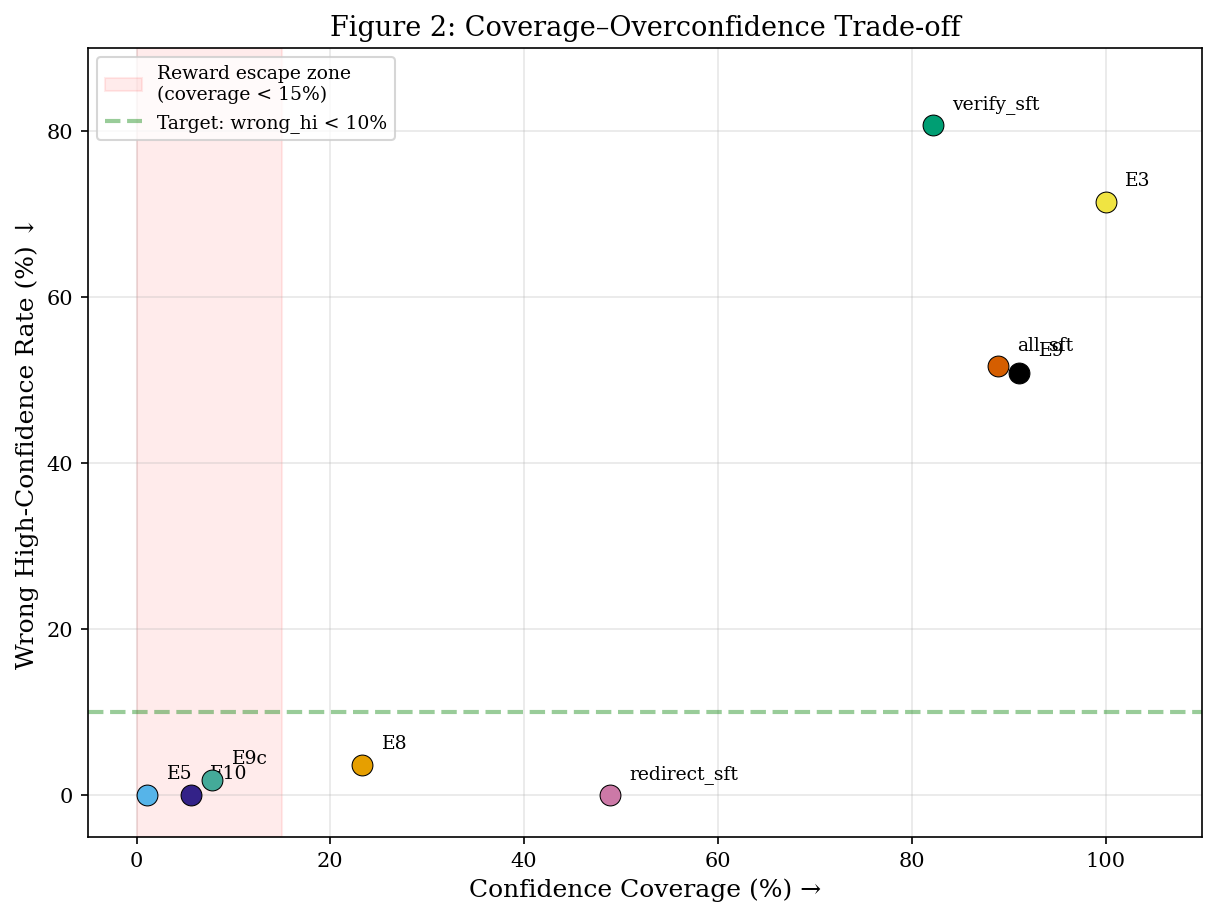
\includegraphics[width=0.85\textwidth]{figures/fig2_coverage_vs_wrong_hi.png}
\caption{Confidence coverage vs.\ wrong high-confidence rate. Red zone indicates reward escape (coverage $<$ 15\%).}
\label{fig:coverage-wronghi}
\end{figure}

\begin{figure}[H]
\centering
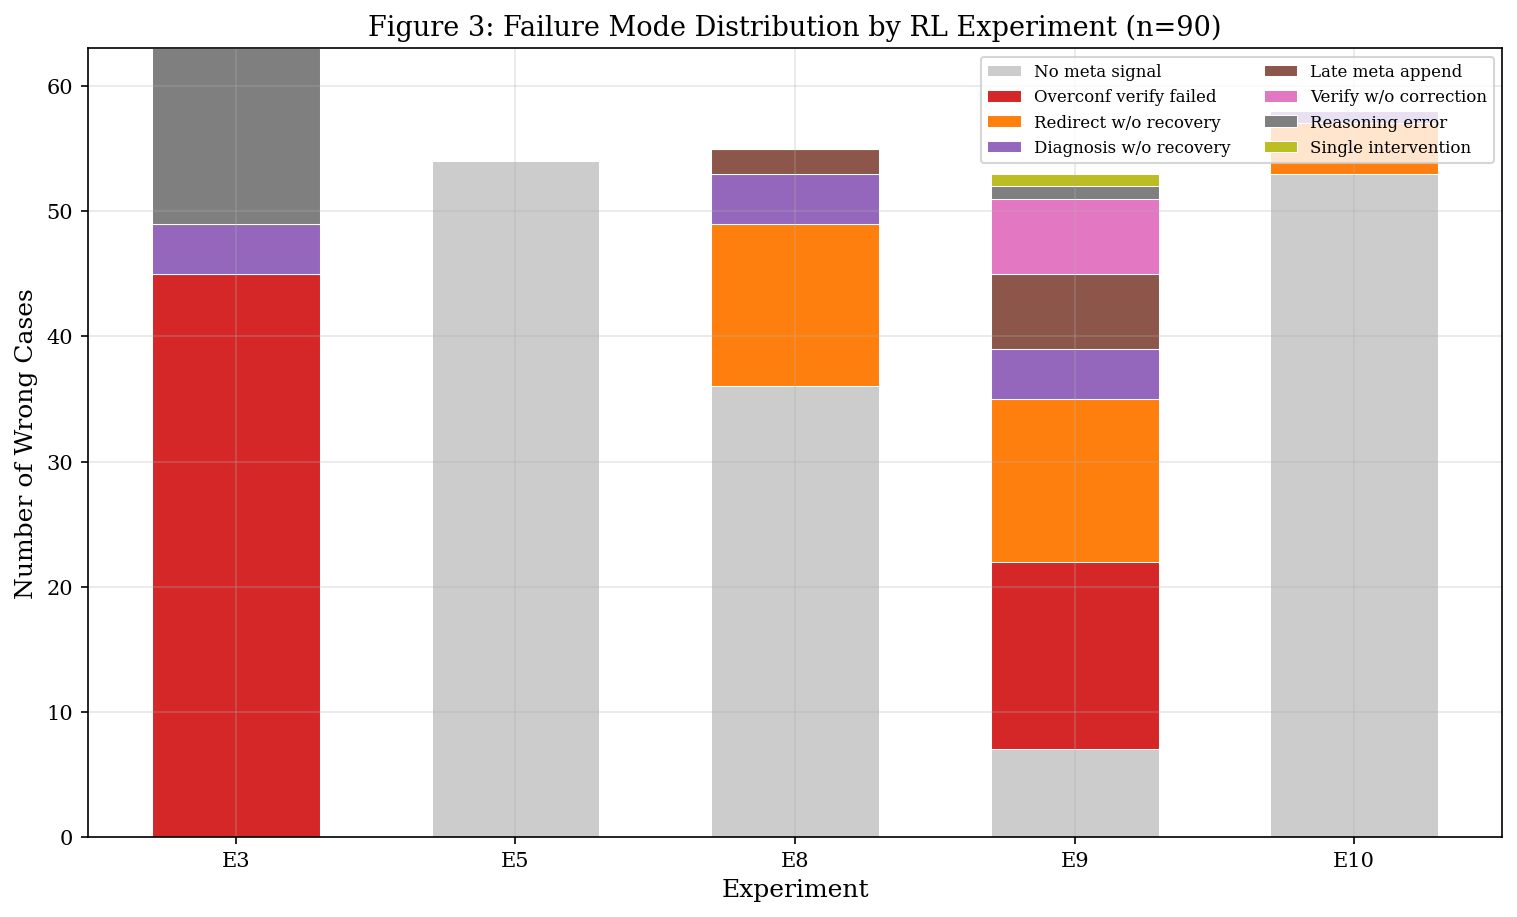
\includegraphics[width=0.85\textwidth]{figures/fig3_failure_modes.png}
\caption{Failure mode distribution across RL experiments (n=90 pilot).}
\label{fig:failure-modes}
\end{figure}

% ──────────────────────────────────────────────────────────────────────
\section{Hypothesis Evaluation}

\subsection{RQ1: Parseable Controller State for OOD Adaptation}

\textbf{Verdict: Weak support.} Meta blocks are parseable across all meta-emitting models. However, no meta model exceeds base\_sft accuracy (42.2 vs.\ 41.1). OOD adaptation is not demonstrated. The controller state is syntactically present but semantically inert.

\subsection{RQ2: Learnability via Reward Decomposition}

\textbf{Verdict: Partial support.}

\begin{itemize}[nosep]
  \item \textbf{Verify (partial):} E9 achieves 90.0 on GSM8K but Wrong\_Hi = 50.9. Verify is decorative.
  \item \textbf{Overconfidence suppression (supported):} E8 reduces Wrong\_Hi to 3.6.
  \item \textbf{Redirect/diagnosis (not supported):} E10 accuracy = 35.6; 53/58 wrong answers have no meta signal.
\end{itemize}

\subsection{RQ3: Curriculum Extensibility}

\textbf{Verdict: Gated.} Diagnosis quality is insufficient for curriculum. Study\_need fields are topically correct but not acted upon. Curriculum gating is maintained until diagnosis-to-recovery $>$ 50\%.

% ──────────────────────────────────────────────────────────────────────
\section{Proposed Improvements}

\subsection{Fix 1: Same-Route Repetition Penalty (Verify Quality)}

\textbf{Problem:} 45/63 wrong answers in E3 and 15/53 in E9 exhibit same-route verify repetition.

\textbf{Solution:} Add a penalty ($-0.5$) when the solve tail after a verify meta block contains repetition language without independent method signals.

\textbf{Expected effect:} Shift verify from paraphrase to independent cross-check; reduce overconfident\_verify\_failed cases.

\subsection{Fix 2: Route-Switch Evidence Reward (Redirect Execution)}

\textbf{Problem:} Redirect meta blocks produce correct diagnoses but subsequent reasoning continues on the original route.

\textbf{Solution:} Add a reward ($+0.9$ correct, $+0.25$ wrong) when the post-redirect solve tail shows structural method difference from the prefix; penalty ($-0.3$) when switch is announced but not evident.

\textbf{Expected effect:} Convert diagnosis-without-recovery to functional redirects.

\subsection{Fix 3: Confidence Omission Floor (Prevent Reward Escape)}

\textbf{Problem:} E5 (1.1\% coverage) and E10 (5.6\%) minimize calibration loss by omitting confidence entirely.

\textbf{Solution:} Penalty ($-0.5$) per completion with zero meta blocks.

\textbf{Expected effect:} Force confidence emission; enable calibration metrics to operate across the full distribution.

% ──────────────────────────────────────────────────────────────────────
\section{Next Experiments}

\subsection{E9v2: Verify with Repetition Penalty}

Applies Fix~1 to E9. \textbf{Hypothesis:} Wrong\_Hi will decrease from 50.9 while GSM8K accuracy stays $\geq$ 85\%. \textbf{Success criterion:} Wrong\_Hi $<$ 30\%; GSM8K $\geq$ 85\%.

\subsection{E9bv2: Redirect with Route-Switch Evidence}

Applies Fix~2 to E9b. \textbf{Hypothesis:} Diagnosis-with-recovery rate will exceed 50\%. \textbf{Success criterion:} Conf\_Cov $\geq$ 30\%; accuracy $\geq$ 38\%.

\subsection{E10v2: Full Controller with All Fixes}

Applies all three fixes to E10. \textbf{Success criterion:} Accuracy $\geq$ 42.2 (base\_sft parity); $\geq$ 2 of 4 failure modes reduced by $\geq$ 50\%.

\subsection{Full-Scale Evaluation Plan}

Models meeting pilot criteria will proceed to the 1,030-problem evaluation (GSM8K 500, MATH-500 500, AIME 30) with \tok{max\_tokens=4096} and deterministic decoding.

\vspace{1em}
\noindent\rule{\textwidth}{0.4pt}

\small
\textit{All numerical results drawn from the Control-V5 pilot evaluation (n=90, 30 per benchmark) unless otherwise noted. Source: \tok{control\_v5\_eval\_readout\_2026\_04\_04.md}}

\end{document}
